% !TEX root = ../vr_st.tex

\section{Example I: Real projective spaces}\label{s:continuous}

For any $n\geq 1$ and $r>0$, let $\bbS^n(r)$ be the $n$-sphere of radius $r$, equipped with the geodesic distance.
The real projective space $\rp^n(r)$ is the quotient space $\bbS^n(r)/\sim$, where $x\sim -x$ for all $x\in \bbS^n $. Let $[x]$ denote the equivalence class of $x$. We equip $\rp^n(r)$ with the quotient metric defined as
\[d_{\rp^n(r)}([x],[x'])=\min \{d_{\bbS^n(r)}(x,x'),d_{\bbS^n(r)}(-x,x')\}.\]
For the simplicity of notation, let $\bbS^n\defeq\bbS^(1)$ and $\rp^n\defeq\rp^n(2)$, so that $\diam\left(\bbS^n \right)=\diam\left(\rp^n \right)=\pi.$

Recall the following results about the homotopy type of the Vietoris--Rips complexes of the spheres and the real projective spaces.
\begin{proposition}\label{prop:homotopy type}
	Let $n\geq 1$.
	\begin{itemize}
		\item[(1)]\label{prop:S1} For any $ t\in \left(\frac{l}{2l+1},\frac{l+1}{2l+3}\right]$, $\VR_t(\bbS^1)$ is homotopy equivalent to $\bbS^{2l+1}$.
		\item[(2)]\label{prop:Sn} For any $ t\in \left(0,\zeta_n\right]$, $\VR_t(\bbS^n)$ is homotopy equivalent to $\bbS^n$, where $\zeta_n\defeq\arccos(\frac{-1}{n+1})$.
		\item[(3)]\label{prop:RPn} For any $ t\in \left(0,\frac{\pi}{3} \right)$, $\VR_t(\rp^n)$ is homotopy equivalent to $\rp^n$.
	\end{itemize}
\end{proposition}

\begin{proof}
	Part (1) appears as Theorem 7.4 of \cite{adamaszek2017vietoris}. Part (2) appears as Theorem 10 of \cite{lim2020vietoris}. Part (3) appears as in Theorem 4.5 of \cite{adams2022metric}.
\end{proof}

The wedge sum $X\vee_{x_0\sim y_0} Y$ (or simply $X\vee Y$) of two pointed metric spaces $(X,x_0)$ and $(Y,y_0)$ is the quotient space of the disjoint union of $X$ and $Y$ by the identification of basepoints $x_0\sim y_0$.
Recall from \cite{burago2001course,adamaszek2020homotopy} that the \emph{gluing metric} on $X\vee Y$ is given by \label{para:gluing}:
$$d_{X\vee Y}(x,y)\defeq d_X(x,x_0)+d_Y(y,y_0),\forall x\in X, y\in Y$$
and $d_{X\vee Y}\vert_{X\times X}=d_X,d_{X\vee Y}\vert_{Y\times Y}=d_Y$.
Recall from \cite[Prop.~3.7]{adamaszek2020homotopy} that the Vietoris--Rips complex of a metric gluing is homotopy equivalent to the wedge sum of the Vietoris--Rips complexes. From this, we deduce that for any degree $p$,
\begin{equation}\label{eq:wedge sum}
	\Hbarc{p}{X\vee Y}= \Hbarc{p}{X}\sqcup \Hbarc{p}{Y}
\end{equation}

\begin{example}[$\bbS^1 \vee \bbS^2$ v.s. $\rp^2$]
	We study the (standard) barcodes and Steenrod barcode of the metric spaces $\bbS^1\vee\bbS^2$ and $\rp^2$. First, because the Vietoris--Rips complexes of these two spaces are contractible for all $t>\pi$, neither the standard barcodes nor the Steenrod barcodes can stay alive after $\pi$. Therefore, all bars are subsets of $(0,\pi)$. \\

	Because of Eq.~(\ref{eq:wedge sum}), to understand the barcodes of $\bbS^1\vee\bbS^2$, it suffices to understand those of $\bbS^1$ and $\bbS^2$. The barcodes of $\bbS^1$ can be obtained from Proposition \ref{prop:homotopy type} (1): for any $l\in \Z_{\geq 0}$,
	\[\Hbarc{2l+1}{\bbS^1}=\left\{\left(\frac{l}{2l+1},\frac{l+1}{2l+3}\right)\right\},\, \Hbarc{2l}{\bbS^1}=\emptyset.\]
	As for the barcodes of $\bbS^2$, first notice that $\Hbarc{1}{\bbS^2}=\emptyset$ \ling{(I need help to explain this. Someone told me the reason during a meeting, but I unfortunately forget the details)}. \facundo{(VR-PH1 of any geodesic metric space is trivial. See papers by Virk. ( The Claim also follows from your own work on persistent homotopy groups.))}\ling{I see!! Thank you.} For degree $2$, it follows from \cite[Proposition 9.4]{lim2020vietoris} that $(0,\zeta_2)\in \Hbarc{2}{\bbS^2}$. Due to the current lack of knowledge about the homotopy types of $\VR_t(\bbS^2)$ for $ t$ close to $\pi$, we are not able to completely characterize the barcodes of $\bbS^2$. But Proposition \ref{prop:homotopy type} (2) tells us that in degree $2$ all bars other than $(0,\zeta_2)$ must be subsets \facundo{(this a bot too generic: why not say must be included in)} of $(\zeta_2,\pi)$, and in degree $p>2$ all bars must be subsets of $(\zeta_2,\pi)$. Combining the above information with Eq.~(\ref{eq:wedge sum}), we obtain (an estimate of) the barcodes of $\bbS^1\vee\bbS^2$, illustrated in the top row of Figure \ref{fig:barcodes}:
	\begin{itemize}
		\item $\Hbarc{1}{\bbS^1\vee \bbS^2}$ contains only one bar $(0,\frac{2\pi}{3})$.
		\item $\Hbarc{2}{\bbS^1\vee \bbS^2}$ contains one bar $(0,\zeta_2)$, and possibly some bars that are subsets of $(\zeta_2,\pi)$;
		\item for any degree $p\geq 3$, the only possible bars in $\Hbarc{p}{\bbS^1\vee \bbS^2}$ are those that are subsets of $(\zeta_2,\pi)$.
	\end{itemize}

	The Steenrod barcodes of $\bbS^1 \vee \bbS^2$ can be estimated and illustrated in the top row of Figure \ref{fig:sq barcodes}, by applying  facts (a) the Steenrod square operation $\Sq^k$ is trivial for the space $\bbS^1\vee\bbS^2$, for any $k\in \Z_{\geq 1}$ and (b) for any $t\in (0,\zeta_2)$, $\VR_t(\bbS^1\vee\bbS^2)$ is homotopy equivalent to $\bbS^1\vee\bbS^2$.
	Indeed, these two facts imply that no Steenrod bars can be born before $\zeta_2$, so they must all be contained in $(\zeta_2,\pi)$. \\

	\begin{figure}
		\centering
		\begin{tabular}{ c c c  }
			\begin{tikzpicture}[scale=0.52]
				\begin{axis} [
					ticklabel style = {font=\Large},
					axis y line=middle,
					axis x line=middle,
					ytick={0.5,0.67,0.95},
					yticklabels={$\frac{\pi}{2}$,$\frac{2\pi}{3}$,$\pi$},
					xtick={0.5,0.67,0.95},
					xticklabels={$\frac{\pi}{2}$,$\frac{2\pi}{3}$,$\pi$},
					xmin=-0.015, xmax=1.1,
					ymin=0, ymax=1.1,]
					\addplot [mark=none] coordinates {(0,0) (1,1)};
					% \addplot [thick,color=black!10!white,fill=black!10!white,
					%                 fill opacity=0.4]coordinates {
						%         (0.67,0.95)
						%         (0.67,0.67)
						%         (0.95,0.95)
						%         (0.67,0.95)};
					\addplot [black!40!white,mark=none,dashed, thin] coordinates {(0,0.67) (0.67,0.67)};
					\addplot [black!40!white,mark=none,dashed, thin] coordinates {(0.67,0) (0.67,0.67)};
					\addplot[barccolor,mark=*] (0, 0.67) circle (2pt) node[above right,barccolor]{\Large\textsf{1}};
					\node[mark=none] at (axis cs:0.68,0.21){$\Hbarc{1}{\bbS^1\vee \bbS^2}$};
				\end{axis}
			\end{tikzpicture}
			&
			\begin{tikzpicture}[scale=0.52]
				\begin{axis} [
					ticklabel style = {font=\Large},
					axis y line=middle,
					axis x line=middle,
					ytick={0.5,0.6,0.67,0.95},
					yticklabels={,$\zeta_2$,,$\pi$},
					xtick={0.5,0.6,0.95},
					xticklabels={$\frac{\pi}{2}$,$\zeta_2$, $\pi$},
					xmin=-0.015, xmax=1.1,
					ymin=0, ymax=1.1,]
					\addplot [mark=none] coordinates {(0,0) (1,1)};
					\addplot [thick,color=black!10!white,fill=black!10!white,
					fill opacity=0.4]coordinates {
						(0.6,0.95)
						(0.6,0.6)
						(0.95,0.95)
						(0.6,0.95)};
					\addplot [black!40!white,mark=none,dashed, thin] coordinates {(0,0.6) (0.6,0.6)};
					\addplot [black!40!white,mark=none,dashed, thin] coordinates {(0.6,0) (0.6,0.6)};
					\addplot[barccolor,mark=*] (0, 0.6) circle (2pt) node[above right,barccolor]{\Large\textsf{1}};
					\node[mark=none] at (axis cs:0.68,0.21){$\Hbarc{2}{\bbS^1\vee \bbS^2}$};
				\end{axis}
			\end{tikzpicture}
			&
			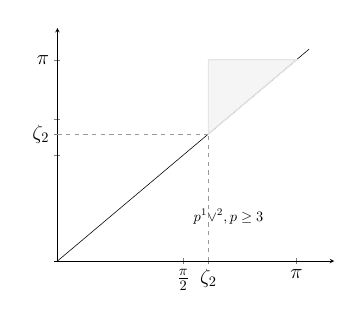
\begin{tikzpicture}[scale=0.52]
				\begin{axis} [
					ticklabel style = {font=\Large},
					axis y line=middle,
					axis x line=middle,
					ytick={0.5,0.6,0.67,0.95},
					yticklabels={,$\zeta_2$,,$\pi$},
					xtick={0.5,0.6,0.95},
					xticklabels={$\frac{\pi}{2}$,$\zeta_2$, $\pi$},
					xmin=-0.015, xmax=1.1,
					ymin=0, ymax=1.1,]
					\addplot [mark=none] coordinates {(0,0) (1,1)};
					\addplot [thick,color=black!10!white,fill=black!10!white,
					fill opacity=0.4]coordinates {
						(0.6,0.95)
						(0.6,0.6)
						(0.95,0.95)
						(0.6,0.95)};
					\addplot [black!40!white,mark=none,dashed, thin] coordinates {(0,0.6) (0.6,0.6)};
					\addplot [black!40!white,mark=none,dashed, thin] coordinates {(0.6,0) (0.6,0.6)};
					\node[mark=none] at (axis cs:0.68,0.21){$\Hbarc{p}{\bbS^1\vee \bbS^2}, p\geq 3$};
				\end{axis}
			\end{tikzpicture}
			\\
			\begin{tikzpicture}[scale=0.52]
				\begin{axis} [
					ticklabel style = {font=\Large},
					axis y line=middle,
					axis x line=middle,
					ytick={0.5,0.67,0.95},
					yticklabels={$\frac{\pi}{2}$,$\frac{2\pi}{3}$,$\pi$},
					xtick={0.5,0.67,0.95},
					xticklabels={$\frac{\pi}{2}$,$\frac{2\pi}{3}$,$\pi$},
					xmin=-0.015, xmax=1.1,
					ymin=0, ymax=1.1,]
					\addplot [mark=none] coordinates {(0,0) (1,1)};
					\addplot [thick,color=black!10!white,fill=black!10!white,
					fill opacity=0.4]coordinates {
						(0.67,0.95)
						(0.67,0.67)
						(0.95,0.95)
						(0.67,0.95)};
					\addplot [black!40!white,mark=none,dashed, thin] coordinates {(0,0.67) (0.67,0.67)};
					\addplot [black!40!white,mark=none,dashed, thin] coordinates {(0.67,0) (0.67,0.67)};
					\addplot[barccolor,mark=*] (0, 0.67) circle (2pt) node[above right,barccolor]{\Large\textsf{1}};
					\node[mark=none] at (axis cs:0.68,0.21){$\Hbarc{1}{\rp^2}$};
				\end{axis}
			\end{tikzpicture}
			&
			\begin{tikzpicture}[scale=0.52]
				\begin{axis} [
					ticklabel style = {font=\Large},
					axis y line=middle,
					axis x line=middle,
					ytick={0.5,0.67,0.95},
					yticklabels={$\frac{\pi}{2}$,$\frac{2\pi}{3}$,$\pi$},
					xtick={0.5,0.67,0.95},
					xticklabels={$\frac{\pi}{2}$,$\frac{2\pi}{3}$,$\pi$},
					xmin=-0.015, xmax=1.1,
					ymin=0, ymax=1.1,]
					\addplot [mark=none] coordinates {(0,0) (1,1)};
					\addplot [thick,color=black!10!white,fill=black!10!white,
					fill opacity=0.4]coordinates {
						(0.67,0.95)
						(0.67,0.67)
						(0.95,0.95)
						(0.67,0.95)};
					\addplot [black!40!white,mark=none,dashed, thin] coordinates {(0,0.67) (0.67,0.67)};
					\addplot [black!40!white,mark=none,dashed, thin] coordinates {(0.67,0) (0.67,0.67)};
					\addplot[barccolor,mark=*] (0, 0.67) circle (2pt) node[above right,barccolor]{\Large\textsf{1}};
					\node[mark=none] at (axis cs:0.68,0.21){$\Hbarc{2}{\rp^2}$};
				\end{axis}
			\end{tikzpicture}
			&
			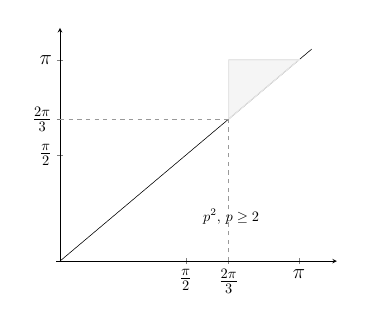
\begin{tikzpicture}[scale=0.52]
				\begin{axis} [
					ticklabel style = {font=\Large},
					axis y line=middle,
					axis x line=middle,
					ytick={0.5,0.67,0.95},
					yticklabels={$\frac{\pi}{2}$,$\frac{2\pi}{3}$,$\pi$},
					xtick={0.5,0.67,0.95},
					xticklabels={$\frac{\pi}{2}$,$\frac{2\pi}{3}$,$\pi$},
					xmin=-0.015, xmax=1.1,
					ymin=0, ymax=1.1,]
					\addplot [mark=none] coordinates {(0,0) (1,1)};
					\addplot [thick,color=black!10!white,fill=black!10!white,
					fill opacity=0.4]coordinates {
						(0.67,0.95)
						(0.67,0.67)
						(0.95,0.95)
						(0.67,0.95)};
					\addplot [black!40!white,mark=none,dashed, thin] coordinates {(0,0.67) (0.67,0.67)};
					\addplot [black!40!white,mark=none,dashed, thin] coordinates {(0.67,0) (0.67,0.67)};
					% \addplot[barccolor,mark=*] (0, 0.67) circle (2pt) node[above right,barccolor]{\Large\textsf{1}};
					\node[mark=none] at (axis cs:0.68,0.21){$\Hbarc{p}{\rp^2},\, p\geq 2$};
				\end{axis}
			\end{tikzpicture}
		\end{tabular}
		\caption{\emph{Top row:} barcodes of $\bbS^1\vee\bbS^2$. \emph{Bottom row:} barcodes of $\rp^2$. In each figure, the gray part is the only region (besides the blue dots) that could contain points in the corresponding barcode. Here, $\zeta_2=\arccos(-\frac{1}3)\approx 0.61\pi$.}
		\label{fig:barcodes}
	\end{figure}

	For the standard barcodes of $\rp^2$, by applying Proposition \ref{prop:homotopy type} (3) and the fact that $\opH_p(\rp^2;\,\Ftwo)$ is $\Ftwo$ for $p=0,1,2$ and $0$ otherwise, we obtain that
	\begin{itemize}
		\item for $p=1,2$, $\Hbarc{p}{\rp^2}$ contains one bar of the form $(0,\beta_p)$ for some $\beta_p\in [\frac{2\pi}{3},\pi]$, and possibly some bars that are subsets of $(\frac{2\pi}{3},\pi)$; \facundo{(would be good to decide on how to describe this " bars that are subsets of.." or "bars that are included in".."bars each of which is contained in.." .. maybe introduce the concept "dominated bars" a bar I = [b,d] is dominated by I' = [b',d'] if $I\subseteq I'$". This brings out more explicitly the poset structure which is often used in AAT)}
		\item for any degree $p\geq 3$, the only possible bars in $\Hbarc{p}{\rp^2}$ are those that are subsets of $(\frac{2\pi}{3},\pi)$.
	\end{itemize}
	\facundo{(seems like the fillingradius should be introduced early on -- before prop 1?)} By \cite[Proposition 9.4]{lim2020vietoris}, $\beta_2$ is equal to twice of the filling radius of $\rp^2$. It is shown in \cite[Theorem 1]{katz1983filling} that the filling radius of $\rp^2$ is $\frac{\pi}{6}$, so we have $\beta_2=\frac{2\pi}{3}$. In addition, we claim that $\beta_1=\frac{2\pi}{3}$. \ling{(This is not finished yet.) First, it follows from the proof of \cite[Proposition 3.5]{adams2022metric} that the simplicial map $h:\VR_t\left(\bbS^2(2)\right)\to \VR_t\left(\rp^2\right)$ defined by $x\mapsto [x]$ induces a homeomorphism $\tilde{h}:\VR_t\left(\bbS^2(2)\right)/\!\sim\,\to \VR_t\left(\rp^2\right)$, where $\sim$ is the equivalence relation induced by identifying the antipodal points. (to continue: argue that the 1-cocycles die when the equilateral triangles are born)
	}

	To compute the Steenrod barcodes of $\rp^2$, we first recall that the only non-trivial Steenrod square operation for the space $\rp^2$ is $\Sq^1$ whose rank is $1$. Indeed, the cohomology ring $\opH^*\left(\rp^2;\,\Ftwo\right)$ is isomorphic to $\Ftwo[\alpha]/(\alpha^3)$ (see \cite[Theorem 3.19]{hatcher2000}) and $\Sq^1(\alpha)=\alpha^2$\footnote{The product operation is the cup product between cohomology classes. When $k$ is the degree of a cohomology class $\alpha$, it is known that $\Sq^k(\alpha)$ is the $k$-fold cup product of $\alpha$ with itself.}. Since the Vietoris--Rips complex $\VR_t\left(\rp^2\right)$ retains the homotopy type of $\rp^2$ for $t\in (0,\frac{2\pi}{3})$, we have one bar in the $\Sq^1$--barcode that is born at $0$ and stay alive until the degree-$2$ class $\alpha^2$ dies at $\frac{2\pi}{3}$. Therefore,
	\begin{itemize}
		\item $\sqbarc{1}{\rp^2}$ contains one bar $(0,\frac{2\pi}{3})$, and possibly some bars that are subsets of $(\frac{2\pi}{3},\pi)$;
		\item for $k\in \Z_{\geq 2}$, the only possible bars in $\sqbarc{k}{\rp^2}$ are those that are subsets of $(\frac{2\pi}{3},\pi)$.
	\end{itemize}

	\begin{figure}
		\centering
		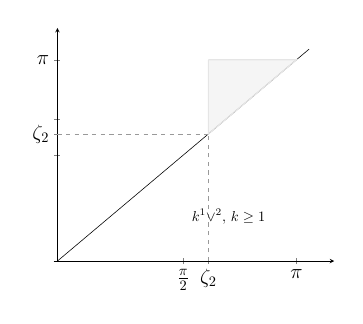
\begin{tikzpicture}[scale=0.52]
			\begin{axis} [
				ticklabel style = {font=\Large},
				axis y line=middle,
				axis x line=middle,
				ytick={0.5,0.6,0.67,0.95},
				yticklabels={,$\zeta_2$,,$\pi$},
				xtick={0.5,0.6,0.95},
				xticklabels={$\frac{\pi}{2}$,$\zeta_2$, $\pi$},
				xmin=-0.015, xmax=1.1,
				ymin=0, ymax=1.1,]
				\addplot [mark=none] coordinates {(0,0) (1,1)};
				\addplot [thick,color=black!10!white,fill=black!10!white,
				fill opacity=0.4]coordinates {
					(0.6,0.95)
					(0.6,0.6)
					(0.95,0.95)
					(0.6,0.95)};
				\addplot [black!40!white,mark=none,dashed, thin] coordinates {(0,0.6) (0.6,0.6)};
				\addplot [black!40!white,mark=none,dashed, thin] coordinates {(0.6,0) (0.6,0.6)};
				\node[mark=none] at (axis cs:0.68,0.21){$\sqbarc{k}{\bbS^1\vee \bbS^2},\, k\geq 1$};
			\end{axis}
		\end{tikzpicture}

		\begin{tikzpicture}[scale=0.52]
			\begin{axis} [
				ticklabel style = {font=\Large},
				axis y line=middle,
				axis x line=middle,
				ytick={0.5,0.67,0.95},
				yticklabels={$\frac{\pi}{2}$,$\frac{2\pi}{3}$,$\pi$},
				xtick={0.5,0.67,0.95},
				xticklabels={$\frac{\pi}{2}$,$\frac{2\pi}{3}$,$\pi$},
				xmin=-0.015, xmax=1.1,
				ymin=0, ymax=1.1,]
				\addplot [mark=none] coordinates {(0,0) (1,1)};
				\addplot [thick,color=black!10!white,fill=black!10!white,
				fill opacity=0.4]coordinates {
					(0.67,0.95)
					(0.67,0.67)
					(0.95,0.95)
					(0.67,0.95)};
				\addplot [black!40!white,mark=none,dashed, thin] coordinates {(0,0.67) (0.67,0.67)};
				\addplot [black!40!white,mark=none,dashed, thin] coordinates {(0.67,0) (0.67,0.67)};
				\addplot[barccolor,mark=*] (0, 0.67) circle (2pt) node[above right,barccolor]{\Large\textsf{1}};
				\node[mark=none] at (axis cs:0.68,0.21){$\sqbarc{1}{\rp^2}$};
			\end{axis}
		\end{tikzpicture}
		\hspace{1.5cm}
		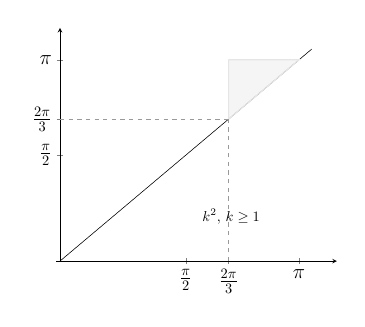
\begin{tikzpicture}[scale=0.52]
			\begin{axis} [
				ticklabel style = {font=\Large},
				axis y line=middle,
				axis x line=middle,
				ytick={0.5,0.67,0.95},
				yticklabels={$\frac{\pi}{2}$,$\frac{2\pi}{3}$,$\pi$},
				xtick={0.5,0.67,0.95},
				xticklabels={$\frac{\pi}{2}$,$\frac{2\pi}{3}$,$\pi$},
				xmin=-0.015, xmax=1.1,
				ymin=0, ymax=1.1,]
				\addplot [mark=none] coordinates {(0,0) (1,1)};
				\addplot [thick,color=black!10!white,fill=black!10!white,
				fill opacity=0.4]coordinates {
					(0.67,0.95)
					(0.67,0.67)
					(0.95,0.95)
					(0.67,0.95)};
				\addplot [black!40!white,mark=none,dashed, thin] coordinates {(0,0.67) (0.67,0.67)};
				\addplot [black!40!white,mark=none,dashed, thin] coordinates {(0.67,0) (0.67,0.67)};
				\node[mark=none] at (axis cs:0.68,0.21){$\sqbarc{k}{\rp^2},\, k\geq 1$};
			\end{axis}
		\end{tikzpicture}

		\caption{\emph{Top row:} Steenrod barcodes of $\bbS^1\vee\bbS^2$. \emph{Bottom row:} Steenrod barcodes of $\rp^2$. }
		\label{fig:sq barcodes}
	\end{figure}
\end{example}

We estimate the bottleneck distance $\db$ between the Steenrod barcodes of the two space $\bbS^1\vee\bbS^2$ and $\rp^2$, and show that it provides a better (lower-bound) approximation of the Gromov-Hausdorff distance than $\db$ between the standard barcodes.

\begin{proposition}\label{prop:db estimate}
	\begin{itemize}
		\item [(1)] $\max_{p\geq 1}\db\left(\Hbarc{p}{\bbS^1\vee\bbS^2}, \Hbarc{p}{\rp^2}\right)\leq \frac{\pi-\zeta_2}{2}\approx 0.2\pi$;
		\item [(2)] $\db\left(\sqbarc{1}{\bbS^1\vee \bbS^2}, \sqbarc{1}{\rp^2}\right)\geq \frac{\pi}{3}.$
	\end{itemize}
\end{proposition}

\begin{proof}
	For Part (1), to prove the bottleneck distance is upper bounded by a value, it is enough to find one matching with cost no larger than this value.

	For degree $1$, consider a matching such that $(0,\frac{2\pi}{3})\leftrightarrow (0,\frac{2\pi}{3})$ and all other points are matched to the diagonal. Then the cost of this matching is at most $\frac{\pi-\frac{2\pi}{3}}{2}=\frac{\pi}{6}< \frac{\pi-\zeta_2}{2}.$
	For degree $2$, consider a matching such that $(0,\zeta_2)\leftrightarrow (0,\frac{2\pi}{3})$ and all other points are matched to the diagonal, whose cost is at most $\max\left\{ \frac{2\pi}{3}-\zeta_2, \frac{\pi-\zeta_2}{2}, \frac{\pi-\frac{2\pi}{3}}{2}\right\} = \frac{\pi-\zeta_2}{2}.$
	For degree $p\geq 3$, consider a matching such that all points are matched to the diagonal, whose cost is at most $\max\left\{ \frac{\pi-\zeta_2}{2}, \frac{\pi-\frac{2\pi}{3}}{2}\right\} = \frac{\pi-\zeta_2}{2}.$
	\\

	For Part (2), recall the $\Sq^1$--barcodes of the two spaces from Figure \ref{fig:sq barcodes}. The bar $(0,\frac{2\pi}{3})$ in $\sqbarc{1}{\rp^2}$ can be mapped to either the diagonal or a point whose first coordinate is larger than or equal to $\zeta_2$. Therefore, a matching between the $\Sq^1$--barcodes will have a cost that is at least $\min\left\{\frac{1}{2}\cdot\frac{2\pi}{3}, \zeta_2\right\} = \frac{\pi}{3}.$
\end{proof}

Proposition \ref{prop:db estimate} shows that the Steenrod barcodes can have a stronger distinguishing power than the standard barcodes in all degrees.
